% Cap�tulo 4


\chapter{Testes de Performance}



Após a fase de construção são aplicados 10 testes de performance no robô. Esses testes levam em consideração o tempo de execução e a quantidade de movimentos que ele faz para chegar a resolução completa do cubo. Cada teste parte de uma configuração inicial, que são um conjunto de peças aleatórias em cada face, até chegar a ordenação dessas peças em cada face correspondente. 

No primeiro conjunto de testes são utilizadas as configurações iniciais mostradas abaixo:

\begin{figure}[htb]
	\centering
  	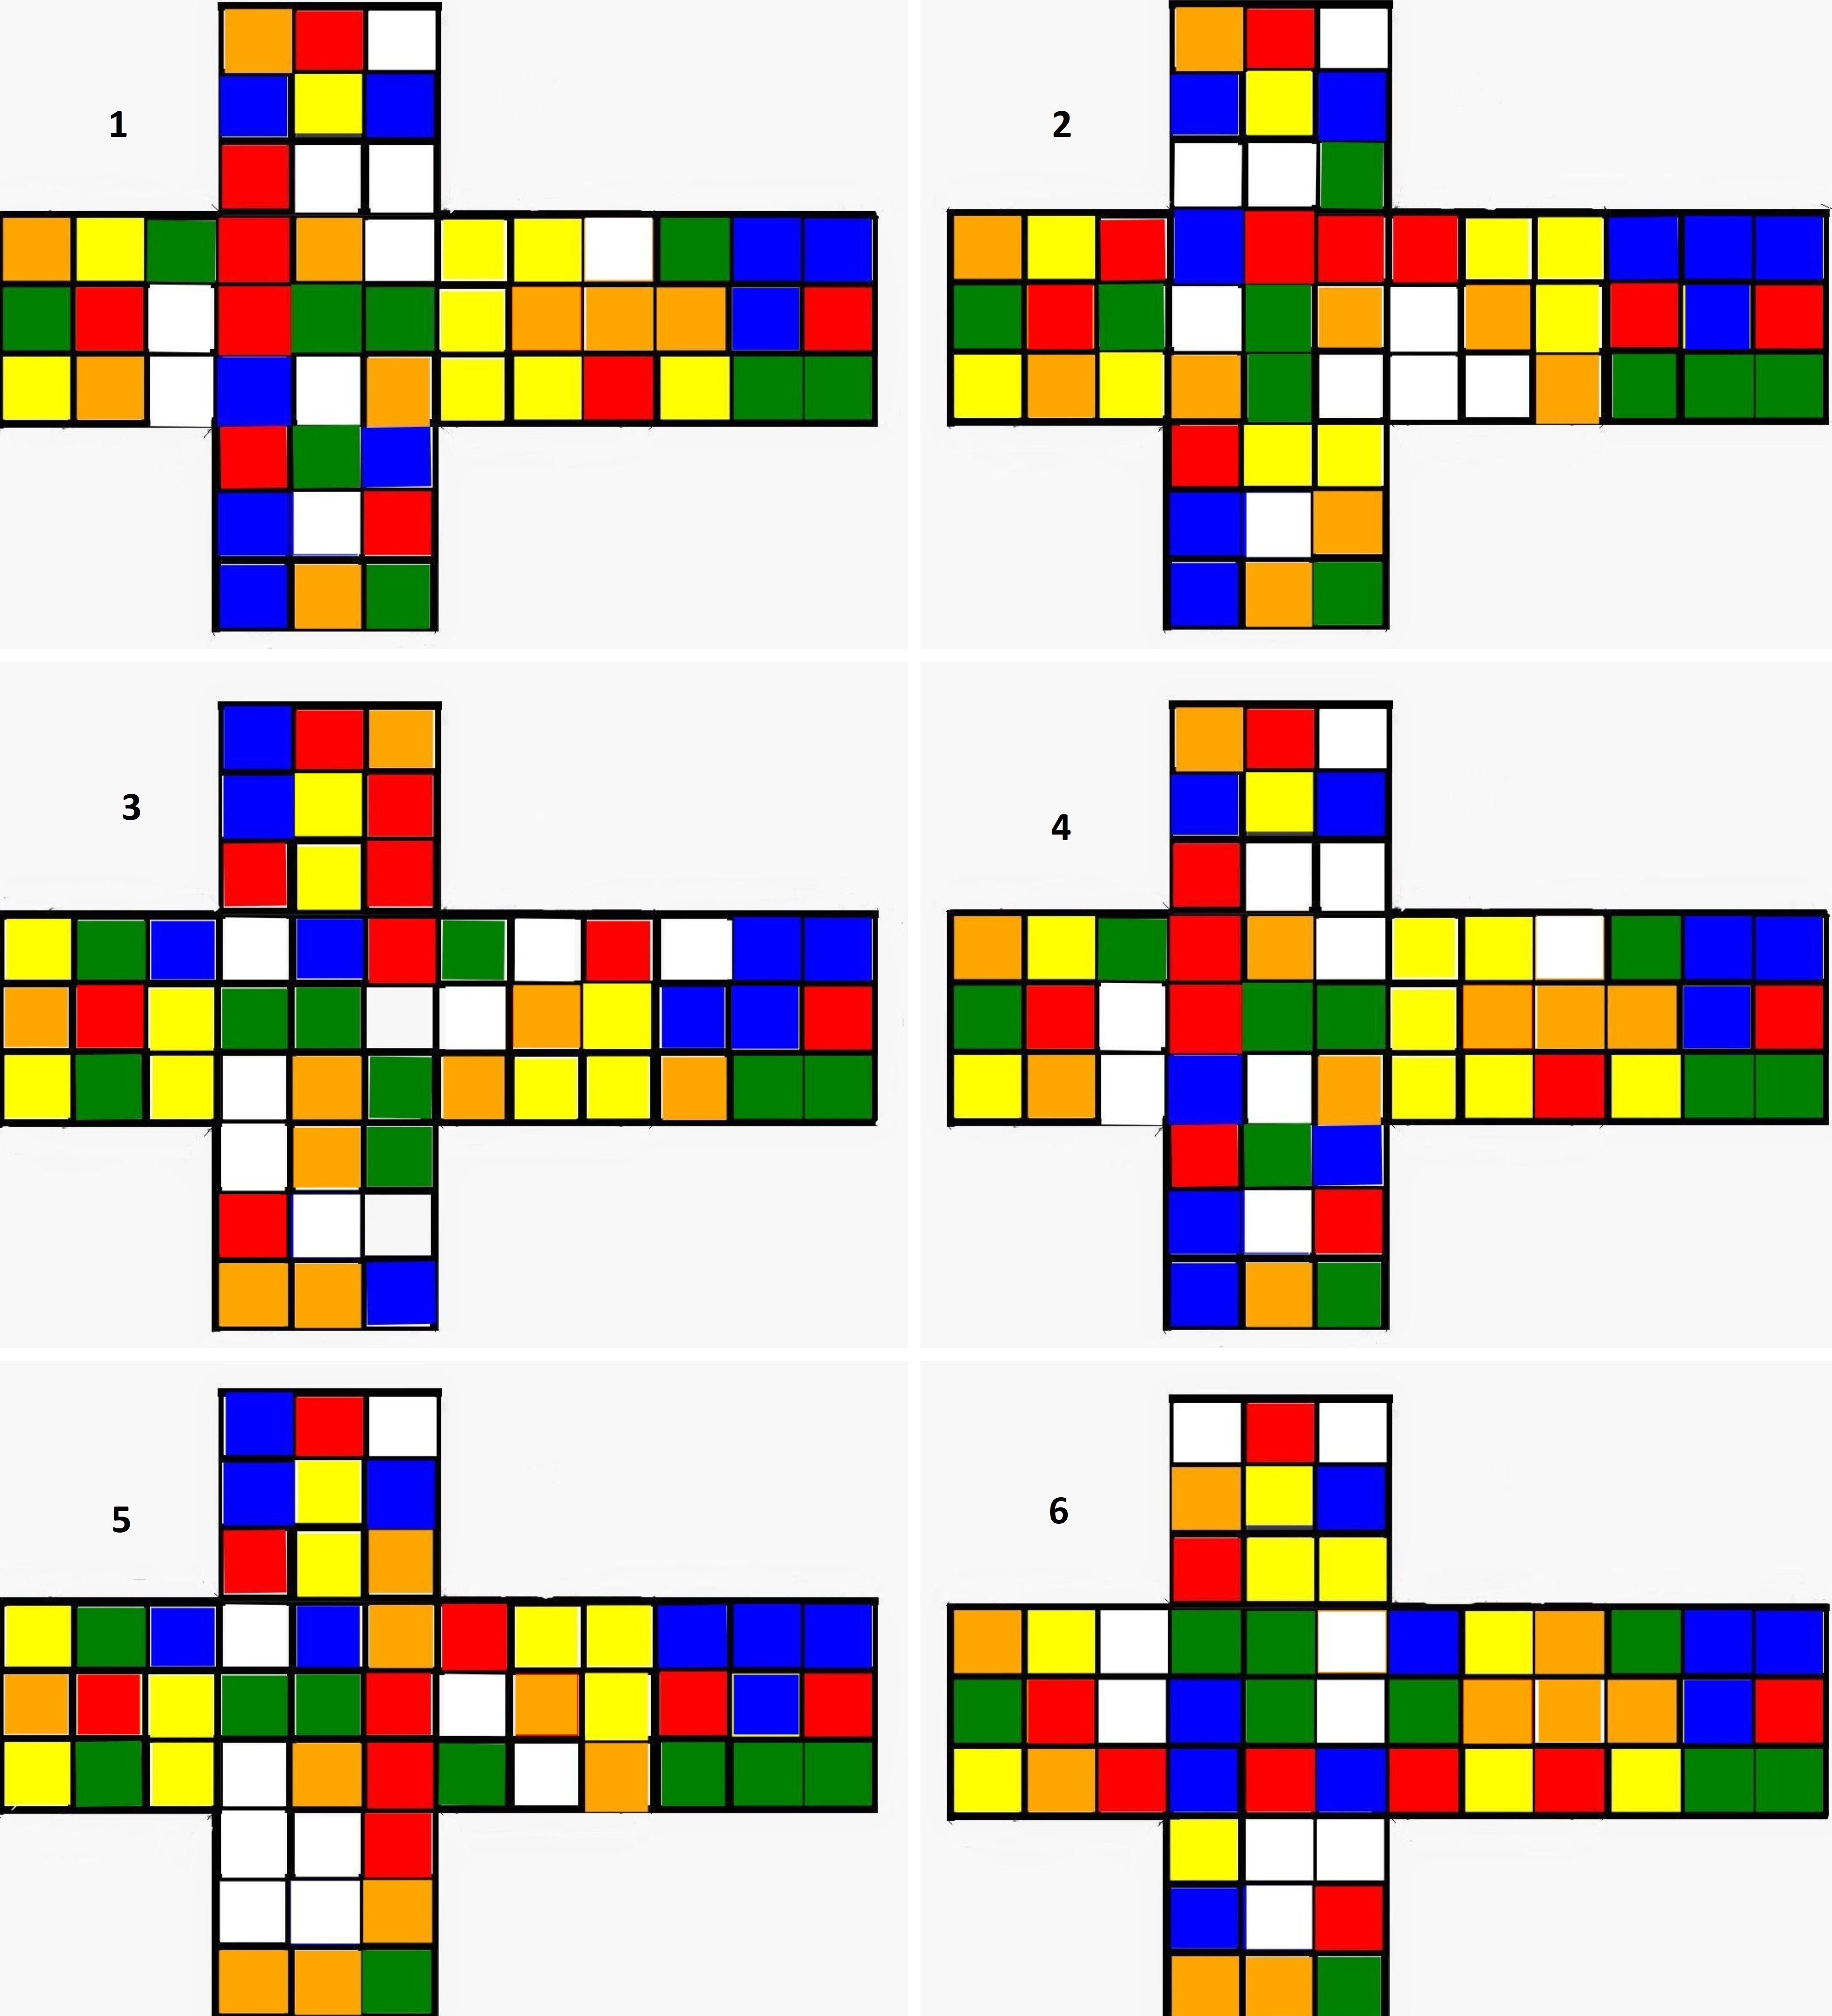
\includegraphics[scale=0.1]{src/imagens/configs1(1).jpg}
  	\textsf{\caption{Conjunto de configurações 1}}
  	\label{fig:FiguraTeste}
\end{figure}



Com este conjunto de configurações, o melhor tempo do robô para chegar a resolução foi 13 minutos, executando um total de 119 movimentos na configuração 1. Já a configuração que precisa de mais tempo é a 6, que precisa de 17 minutos e 36 segundos com um total de 176 movimentos. As outras configurações do conjunto, estão na faixa dos 14 a 15 minutos, aproximadamente, executando entre 139 a 157 movimentos.

No segundo conjunto de configurações, mostrado abaixo, o melhor tempo foi 13 minutos e 20 segundos com um total de 123 movimentos na configuração 10. O robô passou mais tempo para resolver a configuração 7, composta por 168 movimentos que são executados em 16 minutos e 58 segundos. As outras configurações também estão na faixa dos 14 a 15 minutos, aproximadamente, executando entre 133 a 168 movimentos.


\begin{figure}[htb]
	\centering
  	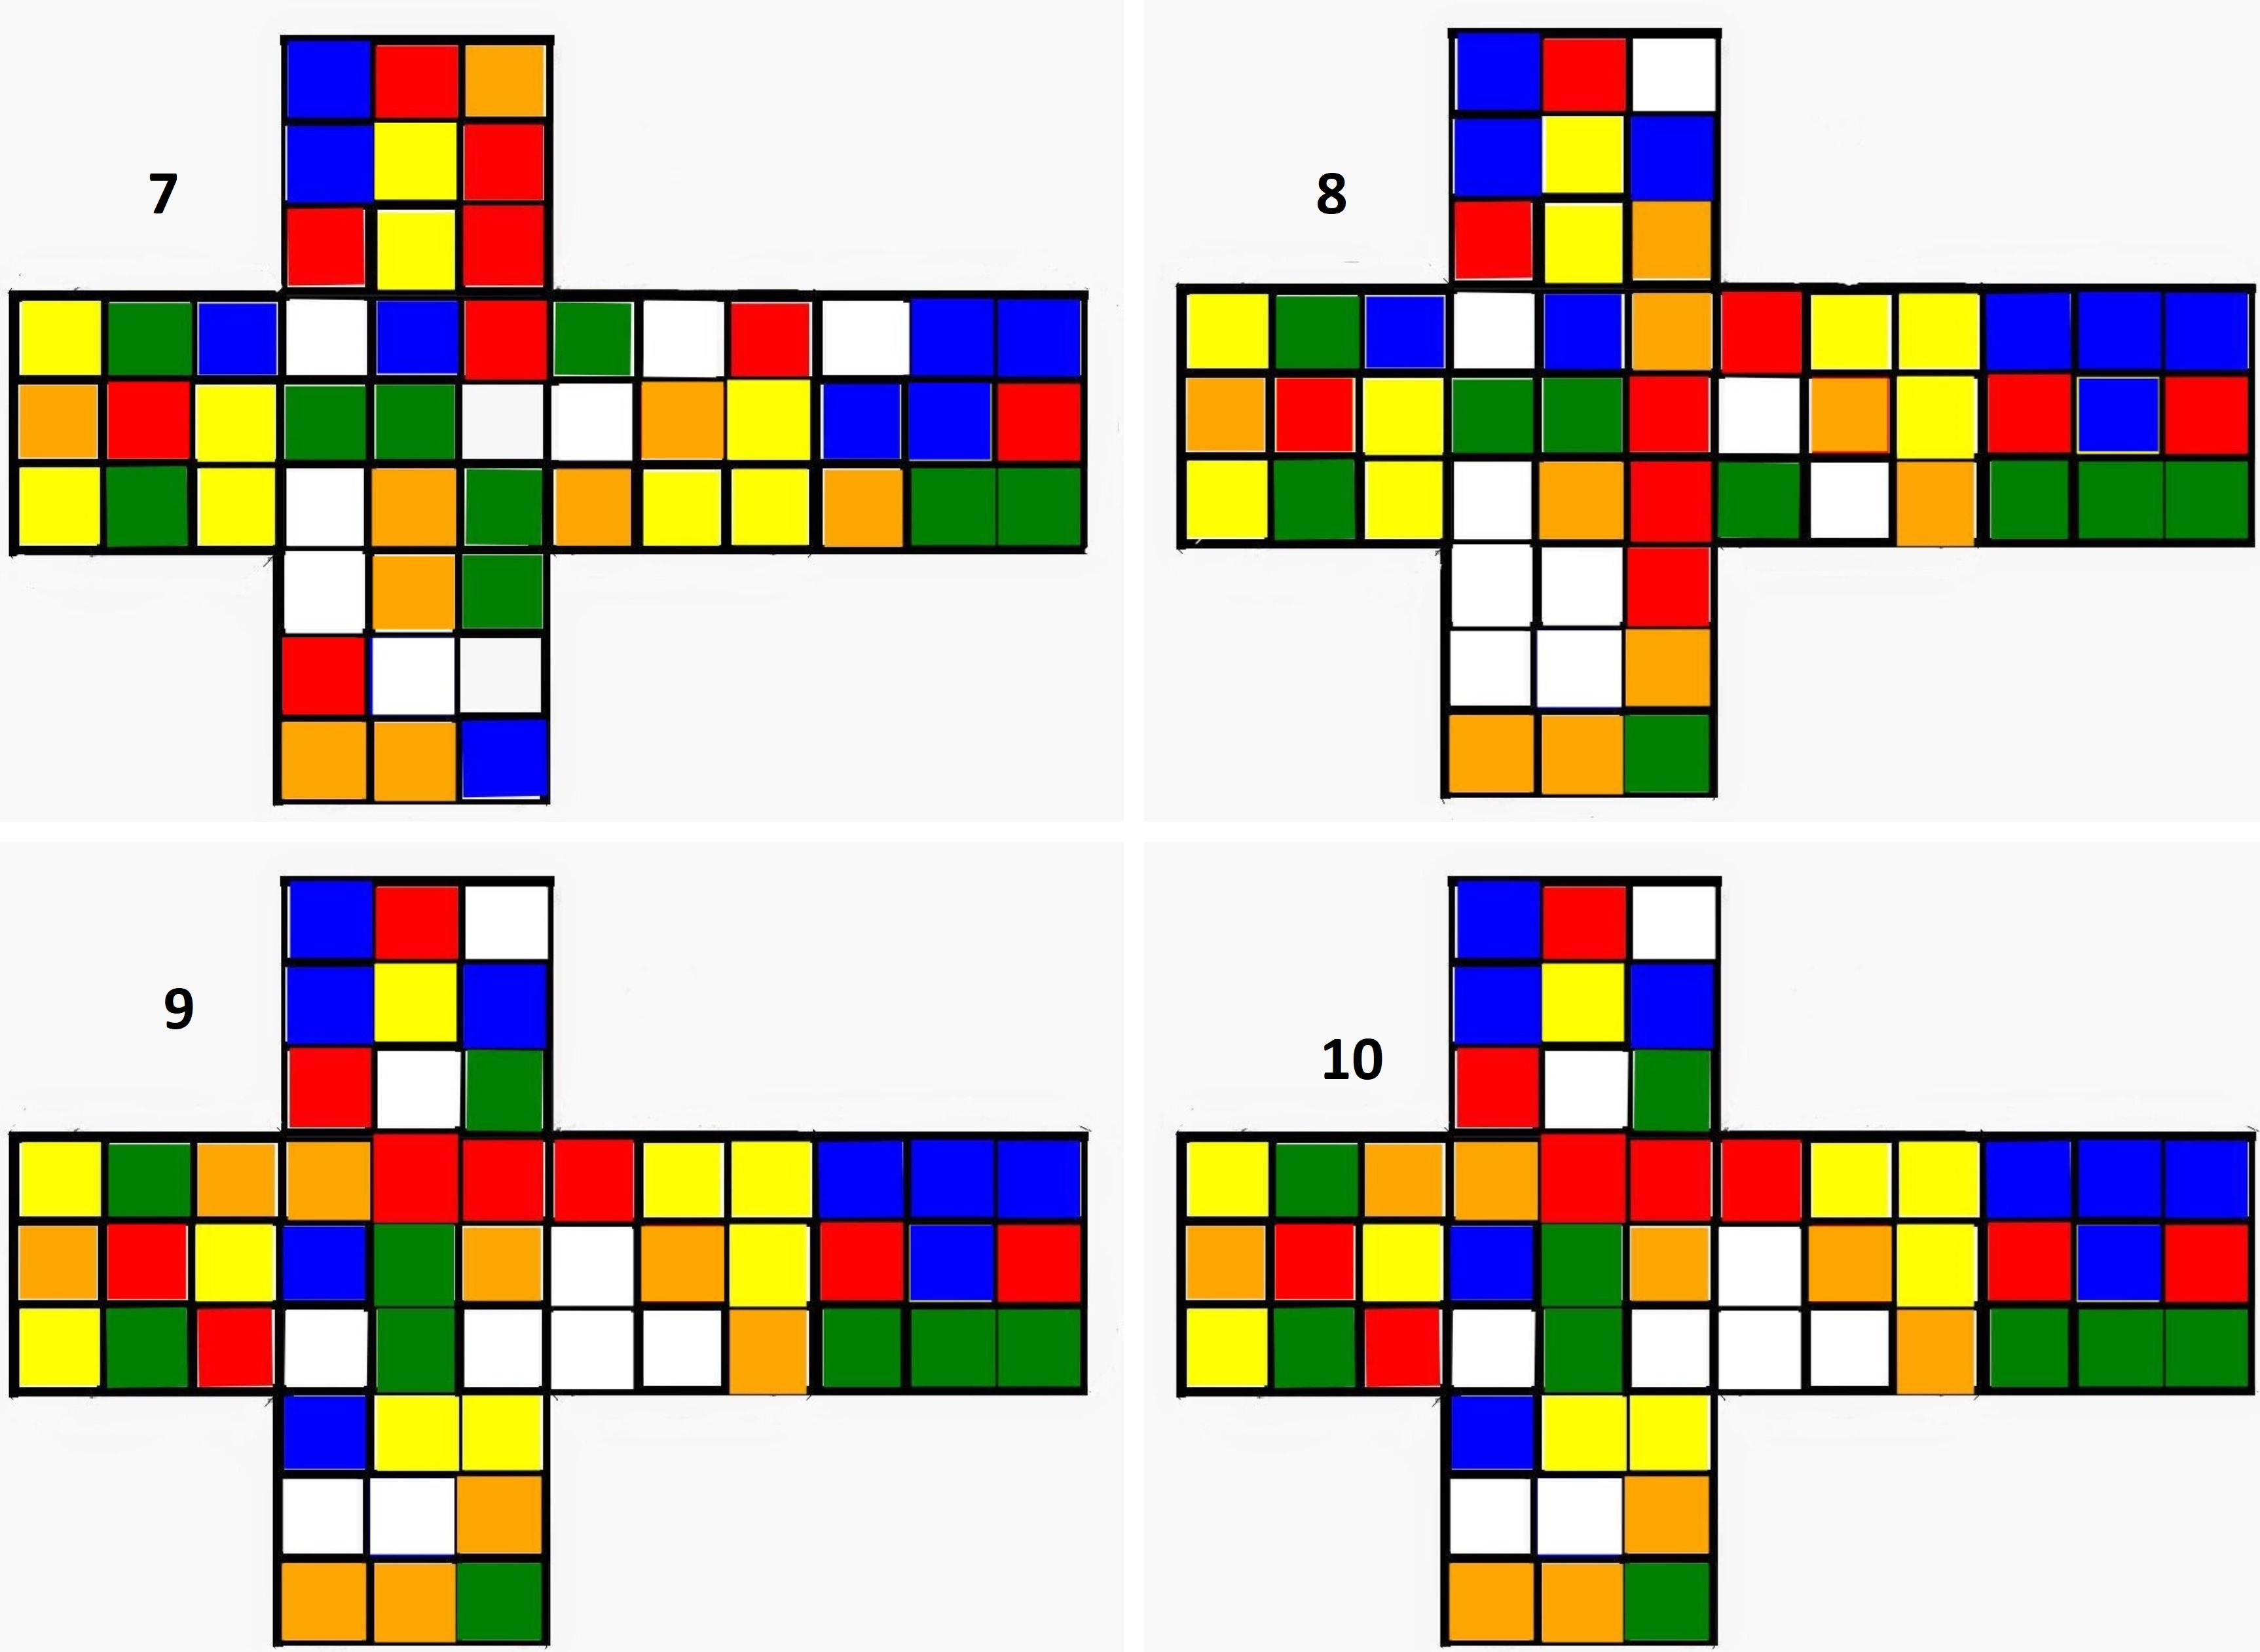
\includegraphics[scale=0.1]{src/imagens/configs2(2).jpg}
  	\textsf{\caption{Conjunto de configurações 2}}
  	\label{fig:FiguraTeste}
\end{figure}




O gráfico abaixo mostra o resultado dos testes das configurações de 1 a 10. É possível perceber que o melhor tempo do robô resolvendo o cubo é 13 minutos. Isso se dá devido a configuração inicial do cubo, quando é preciso executar mais movimentos que envolvam a base, o robô soluciona o cubo de maneira mais rápida. Já as configurações que envolvem mais movimentos do braço mecânico, precisam de mais tempo, pois o braço saí da posição inicial, empurra o cubo e depois volta para sua posição inicial. Essas configurações são mais complexas, por isso o tempo pode chegar a um pouco mais de 17 minutos.

\begin{figure}[htb]
	\centering
  	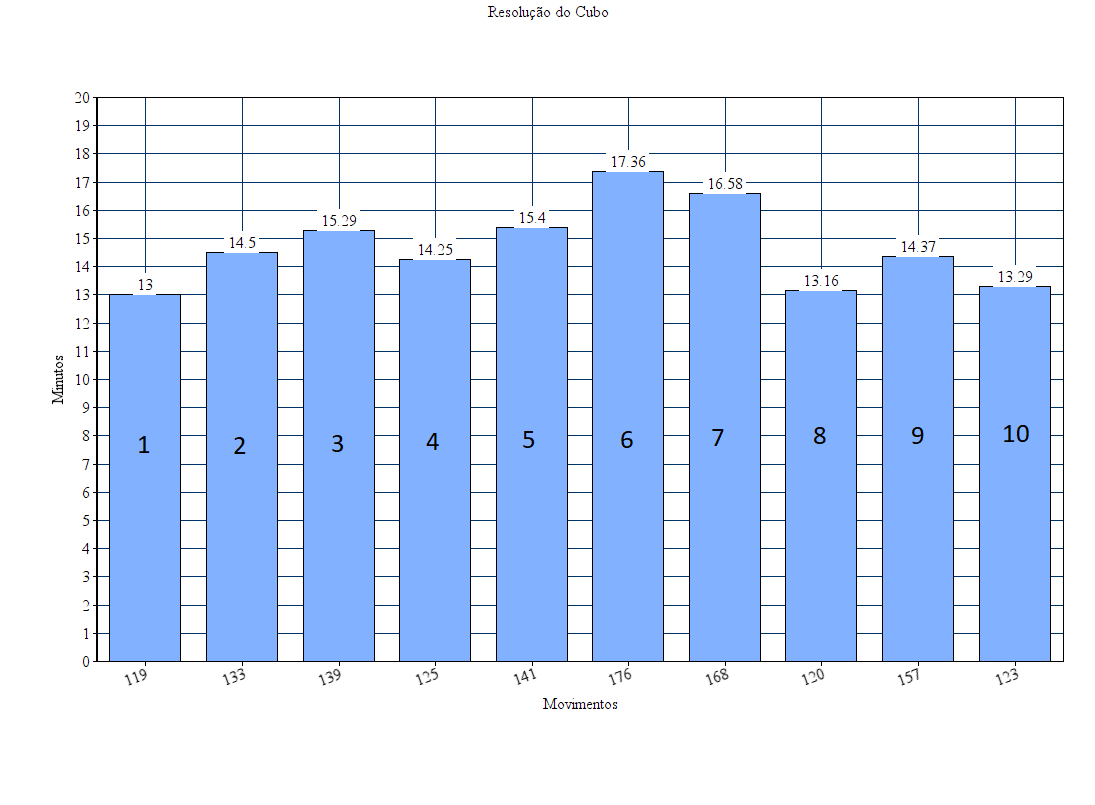
\includegraphics[scale=0.55]{src/imagens/grafico2.png}
  	\textsf{\caption{Gráfico de resultado dos testes}}
  	\label{fig:FiguraTeste}
\end{figure}